\documentclass[a4paper,10pt]{article}
%\usepackage[T1]{fontenc}
\usepackage[utf8]{inputenc}
\usepackage{lmodern}
\usepackage{fancyvrb}
\usepackage{listings}
\usepackage{pdfpages}
\usepackage{graphicx}
\usepackage{array}
\usepackage{float}
\usepackage[dutch]{babel}
\usepackage{lscape}
\usepackage{skak}
\usepackage{algorithm} %ctan.org\pkg\algorithms
\usepackage{algpseudocode}
\usepackage[backend=bibtex8,style=authoryear]{biblatex}
\bibliography{citations}

\newcommand{\code}[1]{\texttt{#1}}
\renewcommand{\contentsname}{Inhoud}
\usepackage[top=1cm, bottom=1cm, left=1cm, right=1cm]{geometry}

%\floatname{algorithm}{Algoritme}
\lstset{
 frame=single,
 breaklines=true,
 postbreak=\raisebox{0ex}[0ex][0ex]{\ensuremath{\color{red}\hookrightarrow\space}}
}

\lstdefinestyle{numbered}{
 numbers=left,               % Ort der Zeilennummern
 stepnumber=1,               % Abstand zwischen den Zeilennummern       
 numberfirstline=false
}


\makeatletter         
\def\@maketitle{
%\raggedright

\includegraphics[width = 50mm]{logo-ugent.pdf}%\\[3ex]
\begin{center}
{\Huge  \@title }\\[4ex] 
{\Large  \@author}\\[4ex] 
\@date\\[8ex]
\end{center}
}


\title{Patbot 2000}
\author{Lissens Tobiah}
\date{2018-06-25}

\begin{document}

\maketitle
\newpage
\newgeometry{top=2cm, bottom=2cm, left=2cm, right=2cm}
\tableofcontents
\newpage


\section{Inleiding}
Schaken is een heel bekende denksport.
Het evalueren van een schaakpositie behoort echter tot de complexiteitsklasse EXPTIME.
Hierdoor is een optimale manier van schaken nog steeds een raadsel.
Dit heeft programmeurs echter niet tegengehouden de uitdaging aan te gaan om schaakcomputers te schrijven die beter zijn dan de menselijke meesters.
Enkele bekende schaakcomputers zijn Stockfish 9, Houdini6 en Alpha Zero.
De bedoeling van dit project is een schaakcomputer te schrijven die gelijkspel kan spelen tegen de schaakcomputer Stockfish 9 met 1 seconde denktijd.
Daarom heeft de schaakcomputer de naam Patbot 2000 toegewezen gekregen. 
 

%----------------------------------------------------------------------------------------
    
\section{Fen Invoer en uitvoer}
    Het parsen van de FEN\footnote{Forsyth-Edwards Notation} gebeurt aan de hand van DCG\footnote{Definite clause grammar}.
    Deze manier van parsen is handig omdat je eenvoudig bidirectioneel kan converteren van FEN-string naar een interne representatie en van een interne representatie terug naar FEN.
    
    \begin{center}
        \newgame
        \fenboard{6R1/K7/8/7k/8/8/8/7R w KQkq - 10 50}
        \showboard
        \\
        \code{FEN 6R1/K7/8/7k/8/8/8/7R w KQkq - 10 50}
    \end{center}
    
    
De bovenstaande matconfiguratie wordt intern met de volgende Prologterm voorgesteld.


    \begin{lstlisting}
        fen_config(
            board(
                row(nil,nil,nil,nil,nil,nil,piece(w,rook),nil),
                row(piece(w,king),nil,nil,nil,nil,nil,nil,nil),
                row(nil,nil,nil,nil,nil,nil,nil,nil),
                row(nil,nil,nil,nil,nil,,nil,piece(b, king)),
                row(nil,nil,nil,nil,nil,nil,nil,nil),
                row(nil,nil,nil,nil,nil,nil,nil,nil),
                row(nil,nil,nil,nil,nil,nil,nil,nil),
                row(nil,nil,nil,nil,nil,nil,nil,piece(w,rook))
            ),w,castle(false,false,false,false),nil,10,50
        )
    \end{lstlisting}
    
De argumenten van fen\_config hebben de volgende betekenis.
\begin{table}[H]
    \caption{}
    \label{tab:Argumenten}
    \begin{center}
        \begin{tabular}{|c|m{10cm}|}
        \hline
        1 Bord & Bord bestaande uit 8 row termen bestaande uit 8 nil of piece(Kleur, Type) termen.\\
        \hline
        2 Kleur & Kleur die op dit moment aan zet is.\\
        3 Rokade & Castle term bestaande uit booleans white kingside, white queenside, black kingside, black queenside respectievelijk.\\
        \hline
        4 Enpassant &  Veld in de voorgaande beurt.\\
        \hline
        5 Halve-zettenteller & telt het aantal zetten sinds het slaan van een stuk of het verzetten van een pion.\\
        \hline
        6 Volle-zettenteller & telt het aantal zetten dat zwart heeft gespeelt sinds  de start van het spel.\\
        \hline
        \end{tabular}
    \end{center}
\end{table}

   
%----------------------------------------------------------------------------------------
\section{Genereren Zetten}
    Het genereren van zetten gebeurt voor de Loper, Toren, Koningin en Koning allemaal op dezelde manier. 
    Dit gebeurt aan de hand van de \code{keep\_moving\_start} regel. Deze kan gevonden worden in file chess\_rules.pl(sectie \ref{chess_rules}) lijn 88.
    In deze regel wordt een lijst van richtingen opgezocht behorende tot het stuktype. Er wordt ook een bereik\footnote{het maximaal aantal vakjes dat ze kunnen opschuiven} meegegeven.
    De richtingen die behoren tot de stukken zijn de volgende: \\
    \begin{table}[H]
        \caption{richtingen}
        \label{tab:}
        \begin{center}
            \begin{tabular}{|c|c|c|}
            \hline
                Stuk & Richtingen & Bereik\\
            \hline
                \symbishop & \code{-1/1, 1/1, -1/-1, 1/-1} & 8\\
            \hline
                \symrook & \code{-1/0, 1/0, 0/-1, 0/-1} & 8\\
            \hline
                \symqueen & \symrook, \symbishop & 8\\
            \hline
                \symking & \symqueen & 1\\
            \hline
            \end{tabular}
        \end{center}
    \end{table}
    Verder kan het paard geïmplementeerd worden door de huidige posite met een positie uit de lijst\\
    \code{[-2/-1, -1/-2, 1/-2, 2/-1, -2/1, -1/2, 1/2, 2/1]} op te tellen.
    De pion bestaat uit heel veel uitzonderingen waarvoor elk een apparte regel is gemaakt deze zijn te vinden in de file chess\_rules.pl (sectie \ref{chess_rules}) vanaf lijn 130.
    Verder word het controleren op schaak staan na een zet gedaan door alle volgende borden te genereren en te controleren of de koning van de huidige kleur nog op het veld staat.
    Deze manier van controleren op schaak is alles behalve efficiënt, maar dit wordt bij het opbouwen van de spelboom bij minimax toch maar uitzonderlijk gebruik van gemaakt.



%----------------------------------------------------------------------------------------
\section{Minimax}
Een implementatie van het minimax algoritme in Prolog wordt uitgelegd in (\cite{minimax}).
Het probleem met gewone minimax toepassen bij schaken is dat deze boom veel te groot zal worden.
We moeten dit dus een klein beetje aanpassen door de spelboom maar tot een bepaalde diepte $d$ op te bouwen.
Wanneer deze diepte $d$ wordt bereikt moeten we een zo goed mogelijke inschatting van de positie kunnen maken.
Dit doen we aan de hand van een heuristische evaluatiefunctie die bepaalt hoe goed een bepaald bord voor de huidige speler is.
Een voorbeeld van een heel slechte maar eenvoudige evaluatie functie is het $\# stukken \ huidige \ speler - \# stukken \ andere \ speler$.


\section{Alpha-Beta} 
Alpha beta snoeien is een verbetering op het minimax algoritme.
Het algoritme werkt door een onder- en bovengrens bij te houden waaraan het beste pad door de spelboom moet voldoen.
Tijdens het algoritme worden deze grenzen geleidelijk aangepast en indien we zeker zijn dat een bepaalde deelbomen niet bezocht moeten worden, kunnen we deze overslaan. 
Het toepassen van het alpha-beta algoritme kan gezien worden in Figuur. \ref{fig:alpha-beta}.
\begin{landscape}
    \begin{figure}
    \begin{center}
        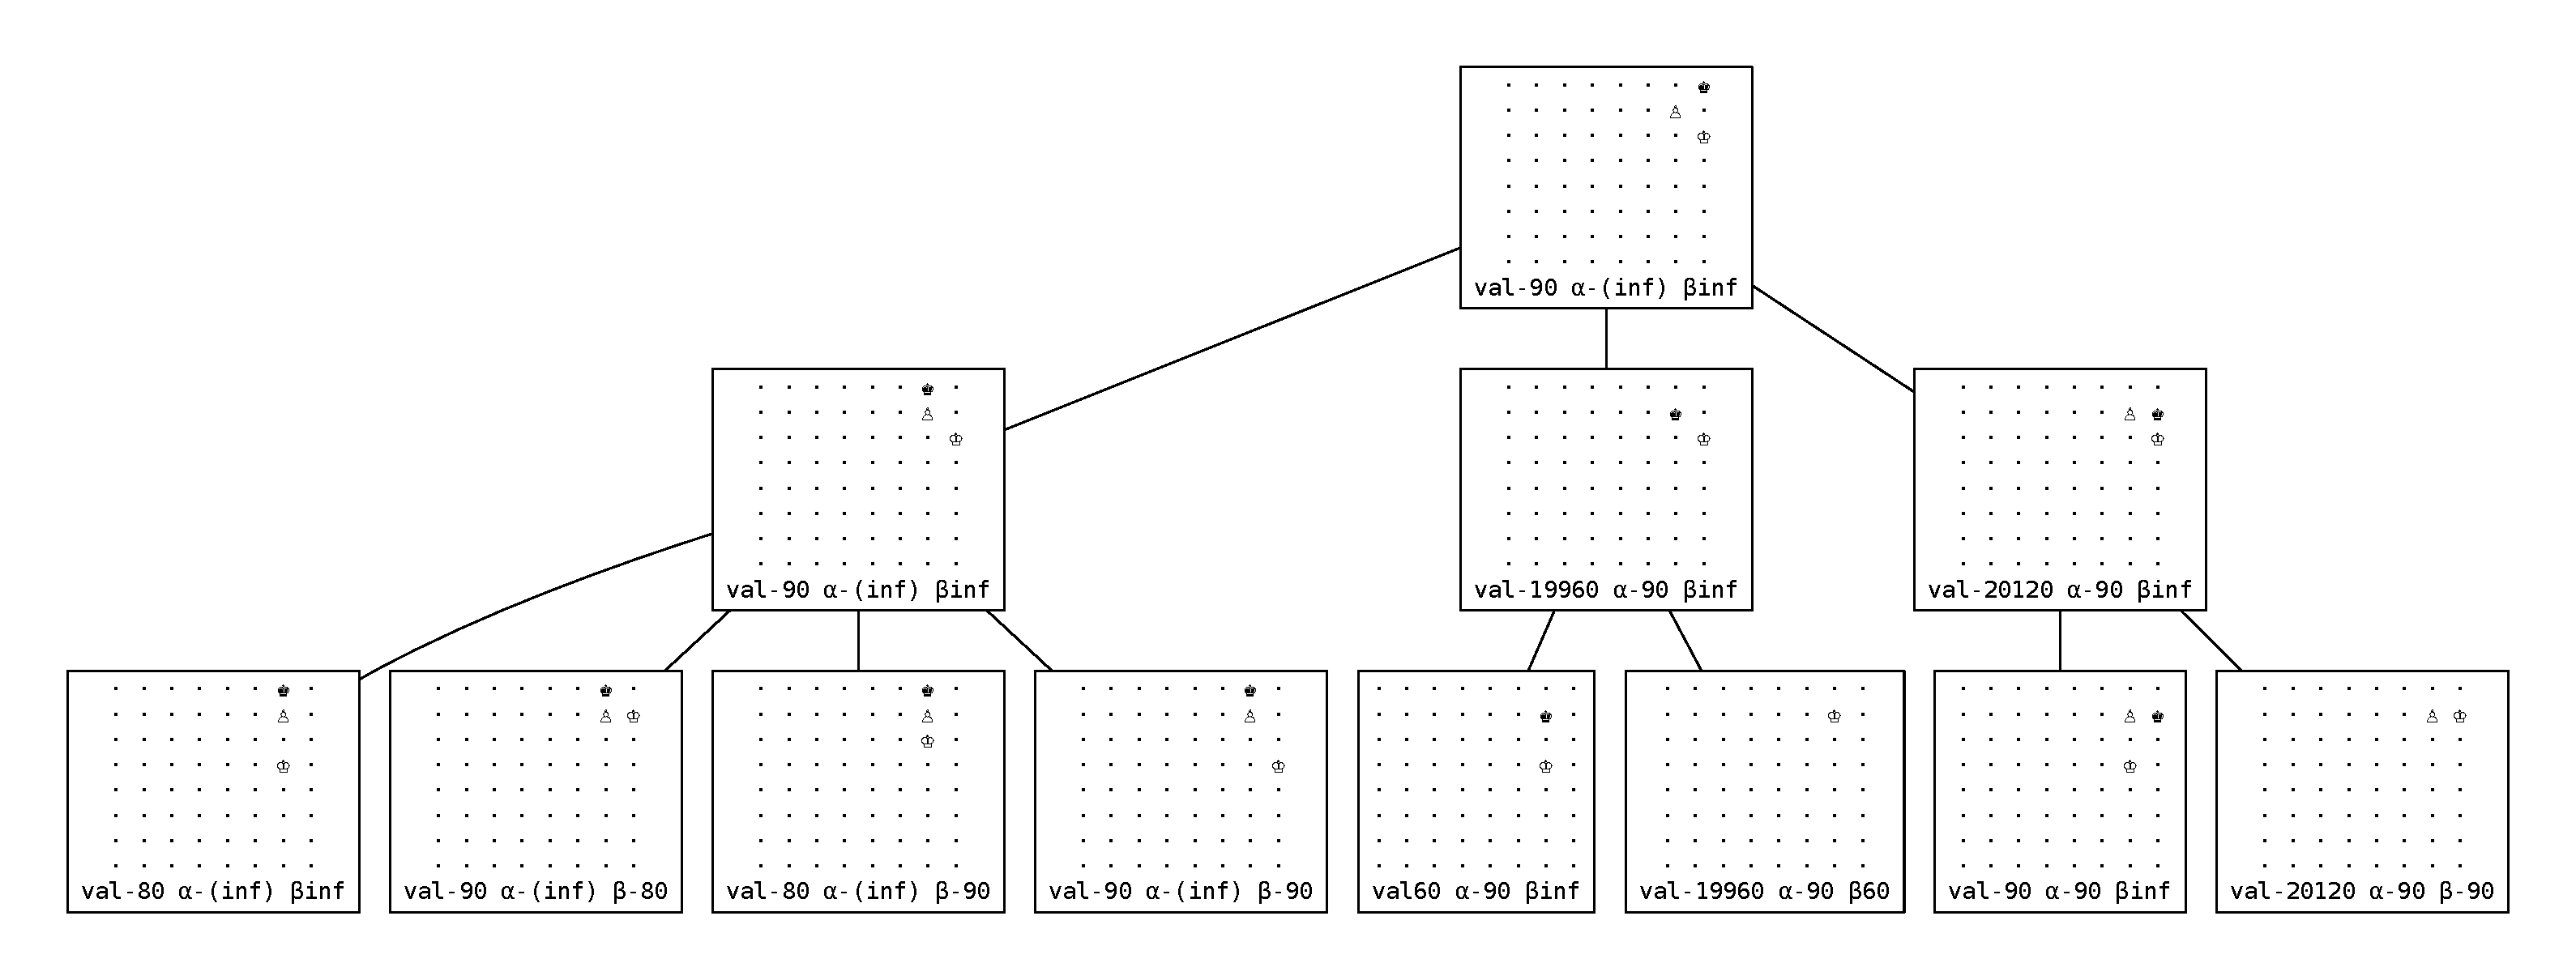
\includegraphics[width=\columnwidth]{coolgraph.pdf}
        \caption{alpha-beta}
        \label{fig:alpha-beta}
    \end{center}
\end{figure}
\end{landscape}


%\begin{algorithm}
%    \caption{Aanpassen grenzen}
%    \begin{algorithmic}[1]
%        \Procedure{grenzen}{\textit{alpha}, \textit{beta}, \textit{value}, \textit{bord}}      
%            \If{\textit{bord} == zelfde kleur wortel bord $\wedge$ \textit{value} $>$ \textit{alpha}}
%                \State \textit{alpha} $\gets$ \textit{value}
%            \ElsIf{\textit{bord} == andere kleur wortel bord $\wedge$ \textit{value} $<$ \textit{beta}}
%                \State \textit{beta} $\gets$ \textit{value}
%            \EndIf               
%        \EndProcedure
%    \end{algorithmic}
%    \label{alg:grenzen}
%\end{algorithm}

%\begin{algorithm}
%    \caption{Snoeien}
%    \begin{algorithmic}[1]
%        \Procedure{snoeien}{\textit{alpha}, \textit{beta}, \textit{value}, \textit{bord}}      
%            \If{\textit{bord} == zelfde kleur wortel bord $\wedge$ \textit{value} $>=$ \textit{beta}}
%                \State \Return{\textit{value}, \textit{bord}} 
%            \ElsIf{\textit{bord} == andere kleur wortel bord $\wedge$ \textit{value} $<=$ \textit{alpha}}
%                \State \Return{\textit{value}, \textit{bord}}
%            \EndIf
%            \State \Return{niet snoeien}          
%        \EndProcedure
%    \end{algorithmic}
%    \label{alg:snoeien}
%\end{algorithm}

Het alpha-beta algoritme in Prolog kan gevonden worden in bestand chess\_alpha\_beta.pl \ref{chess_alpha_beta} gebaseerd op (\cite{alpha-beta}).


%----------------------------------------------------------------------------------------
\section{Evaluatie}
 Bij het afkappen van een zoekboom op een zeker diepte moeten we een positie kunnen evalueren.
 Het kiezen van een goede evaluatie functie is enorm belangrijk.
 In deze implementatie hebben we gekozen voor de simplified chess evaluatie functie die in (\cite{evaluation}) staat beschreven.
 Het komt er op neer dat elk stuk de waarde zoals in Tabel \ref{tab:waarden} wordt toegekend.
 De meeste waarden zijn vanzelfsprekend behalve deze voor het paard en de loper. 
 De meeste schaakboeken kennen deze elk een score van 300 toe, maar om te voorkomen dat deze stukken worden geruild voor 3 pionen. 
 En om er voor te zorgen dat een loper paar meer waard is dan een paarden paar krijgen deze een iets hogere score waarde.
 Ook wordt de score van de koning in de tabel opgenomen. Hierdoor moeten we tijdens het berekenen van de volgende stukken niet meer expleciet op schaak controleren wat een relatief dure operatie is.
 De bovenstaande manier van werken wordt semi-legale-zettengeneratie genoemd.
 \begin{table}[H]
     \begin{center}
         \begin{tabular}{|c|c|}
         \hline
                stuk & waarde \\
         \hline
               \sympawn & 100 \\
         \hline
               \symknight & 320 \\
         \hline
               \symbishop & 330 \\
         \hline
               \sympawn & 500 \\
         \hline
               \symqueen & 900 \\
         \hline
               \symking & 20000\\
         \hline
         \end{tabular}
     \end{center}
     \caption{Waarden van stukken}
     \label{tab:waarden}
 \end{table}
    
Verder is bij het evalueren ook de positie van de stukken belangrijk: het aantal velden dat ze bedreigen en het samenhangen van pionnen enzovoort.
Hiervoor wordt er gebruik gemaakt van positie tabellen. Dit zijn tabellen die voor elke coördinaat een bonus waarde of penalty toekennen.
Zoals we bijvoorbeeld in \ref{chess_evaluation} lijn 90 kunnen zien, krijgt een paard een grote bonus wanneer hij in het midden staat. Terwijl hij een grote panalty krijgt wanneer hij in de hoek staat.
Dit komt doordat een paard in het midden 8 velden kan bereiken terwijl een paard in een hoek er maar 2 kan bereiken.

%----------------------------------------------------------------------------------------

\section{Resultaten} 
In Tabel.\ref{tab:result} zien we Patbot 2000 die zowel tegen stockfish 9 als tegen pychess(bot van pychess ) 6 games speelt (3 keer zwart 3 keer wit).
Zowel pychess als stockfish kregen alletwee maar 1 seconde denktijd voor een zet.
Zoals verwacht presteren zowel stockfish als pychess zelfs met de beperkte denktijd veel beter.

\begin{table}[H]
    \caption{Resultaten op 5 games}
    \label{tab:result}

    \begin{center}
        \begin{tabular}{|c|c|c|c|}
            \hline
           match & win eerste & win tweede & draw \\
           \hline
           pychess vs Patbot 2000  & 4 & 0 & 2\\
            \hline
           stockfish 9 vs Patbot 2000  & 6 & 0 & 0\\
           \hline
           stockfish 9 vs pychess  & 6 & 0 & 0 \\
            \hline
        \end{tabular}
    \end{center}
\end{table}

\section{Bespreking}
De huidig Patbot heeft echter nog heel wat gebreken. Enkele mogelijke verberteringen zijn de volgende.
Patbot kan op dit moment geen onderscheid maken tussen verschillende gamefases zoals het begin, midden of einde.
We zouden een heuristiek kunnen schrijven die de huidige gamefase bepaalt door bijvoorbeeld het aantal aanwezige stukken te tellen.
Aan de hand van de gamefase zouden we dan onze pos/stuk-score kunnen aanpassen.
Een koning in de begin-en middenfase aan de rand is goed, maar in het eindspel is het meestal voordelig deze meer in het spel te betrekken.
Verder maakt de huidige schaakcomputer ook nog gebruik van semi-legale-zettengeneratie. Dit wil zeggen dat we bij het genereren van de volgende zetten in de spelboom niet checken of de koning schaak staat. Het probleem hiermee is dat wanneer de schaakbot zijn tegenstander mat wilt zetten hij het verschill tussen mat en pat niet kan opmerken.
Door het gebruik van de gamefases zouden we in het eindspel kunnen overschakelen naar legale move generatie. Controleren op schaak staan is een grote kost maar in het eindspel is het aantal mogelijke zetten ook een stuk kleiner.
Er zijn echter nog vele andere mogelijke technieken uit de computerschaakwereld die kunnen toegepast worden maar de bovenstaande zijn kleine modificaties aan de huidige Patbot die het programma toch al een stuk beter kunnen maken.

%----------------------------------------------------------------------------------------
\section{Conclusie}% nog wat meer zever
Zoals verwacht is het schrijven van een goede schaakcomputer een hele grote uitdaging die buiten de scope van dit vak ligt.
Het is dus ook logisch dat deze schaakcomputer niet heel goed presteert.
Desalnietemin is deze schaakcomputer een mooi proof of concept en heel handig om verschillende concepten uit de schaakcomputerwereld snel uit te proberen.



\section{Bedanking}
Graag zou ik Ruben Maes willen bedanken, die een fen2uci wrapper heeft geschreven, hiermee was het eenvoudig de bot te koppelen aan GUI's of andere bots. 
%----------------------------------------------------------------------------------------
%	REFERENCE LIST
%----------------------------------------------------------------------------------------
\printbibliography
%----------------------------------------------------------------------------------------


\newgeometry{top=2cm, bottom=2cm, left=1cm, right=1cm}
\section{Appendix Broncode}
  \subsection{Src}
    \subsubsection{main.pl}\label{main}
      \lstinputlisting[style=numbered]{../src/main.pl}
    \subsubsection{chess\_io.pl}\label{chess_io}
      \lstinputlisting[style=numbered]{../src/chess_io.pl}
    \subsubsection{chess\_operations.pl}\label{chess_operations}
      \lstinputlisting[style=numbered]{../src/chess_operations.pl}
    \subsubsection{chess\_rules.pl}\label{chess_rules}
      \lstinputlisting[style=numbered]{../src/chess_rules.pl}
    \subsubsection{chess\_engine.pl}\label{chess_engine}
      \lstinputlisting[style=numbered]{../src/chess_engine.pl}
    \subsubsection{chess\_alpha\_beta.pl}\label{chess_alpha_beta}
      \lstinputlisting[style=numbered]{../src/chess_alpha_beta.pl}
    \subsubsection{chess\_evaluation.pl}\label{chess_evaluation}
      \lstinputlisting[style=numbered]{../src/chess_evaluation.pl}
  \subsection{Test}
    \subsubsection{test\_main.pl}\label{test_main}
        \lstinputlisting[style=numbered]{../test/test_main.pl}
    \subsubsection{test\_chess\_io.pl}\label{test_chess_io}
        \lstinputlisting[style=numbered]{../test/test_chess_io.pl}
    \subsubsection{test\_chess\_rules.pl}\label{test_chess_rules}
        \lstinputlisting[style=numbered]{../test/test_chess_rules.pl}
    \subsubsection{test\_chess\_util.pl}\label{test_chess_util}
        \lstinputlisting[style=numbered]{../test/test_chess_util.pl}
  \restoregeometry
\end{document}
